%%%%%%%%%%%%%%%%%%%%%%%%%%%%%%%%%%%%%%%%%%%
%%% DOCUMENT PREAMBLE %%%
\documentclass[12pt]{article}

\newcommand\attr[2]{%%
  \expandafter\def\csname#1\endcsname{#2}%%
}

\newcommand{\firstpage}{
  \begin{titlepage}
    \centering
      \vspace*{0.5 cm}
    \begin{center}    \textsc{\Large \university}\\[2.0 cm]	\end{center}% University Name
    \textsc{\Large \mastertheme }\\[0.5 cm]				% Course Code
    \rule{\linewidth}{0.2 mm} \\[0.4 cm]
    { \huge \bfseries \thetitle}\\
    \rule{\linewidth}{0.2 mm} \\[1.5 cm]

    \begin{minipage}{0.4\textwidth}
      \begin{flushleft} \large
        \end{flushleft}
        \end{minipage}~
        \begin{minipage}{0.4\textwidth}

        \begin{flushright} \large
          \emph{Student:} \\
          \author \\
          \emph{Professor:} \\
          \professor
      \end{flushright}

    \end{minipage}\\[2 cm]

    \includegraphics[scale = 0.5]{imgs/\universityinitials.png}
  \end{titlepage}
}

\usepackage{agda}
\usepackage{hyperref}
\usepackage{apacite}
\usepackage{catchfilebetweentags}

\usepackage{ucs}
\usepackage{amssymb}

\usepackage[english]{babel}
\usepackage{url}
\usepackage[utf8x]{inputenc}
\usepackage{amsmath}
\usepackage{graphicx}
\graphicspath{{imgs/}}
\usepackage{parskip}
\usepackage{fancyhdr}
\usepackage[acronym]{glossaries}
\usepackage[final]{pdfpages}

\usepackage{vmargin}
\setmarginsrb{3 cm}{2.5 cm}{3 cm}{2.5 cm}{1 cm}{1.5 cm}{1 cm}{1.5 cm}
\newcommand{\agda}[2]{\ExecuteMetaData[latex/#1.tex]{#2}}
\newcommand{\incgraph}[2]{\includegraphics[width=\columnwidth/#2]{#1}}
\newcommand{\incimgdiv}[4]{
  \begin{figure}
    \incgraph{#1.#2}{#4}
    \caption{#3}
    \label{fig:#1}
  \end{figure}
}
\newcommand{\incimg}[3]{\incimgdiv{#1}{#2}{#3}{1}}
\newcommand{\figref}[1]{Figure \ref{fig:#1}}
\newcommand{\subtitle}[1]{{\large \textbf{#1}}}
\newcommand{\initial}[2]{\textbf{#1:} #2 \\}
\newcommand{\plabel}[1]{
\phantomsection
\label{#1}
}


\makenoidxglossaries
\newacronym{pow}{PoW}{Proof-of-Work}
\newacronym{utxo}{UTXO}{Unspent Transaction Output}
\newacronym{pos}{PoS}{Proof of Stake}
\newacronym{rsa}{RSA}{Rivest Shamir Adleman}
\newacronym{sha}{SHA-256}{Secure Hash Algorithm 2}
\newacronym{cpu}{CPU}{Central Processing Unit}
\newacronym{id}{ID}{Identity}
\newacronym{dao}{DAO}{Decentralized Autonomous Organization}
\newacronym{kzsnark}{zk-SNARK}{Zero-Knowledge Succinct Non-Interactive Argument of Knowledge}
\newacronym{evm}{EVM}{Ethereum Virtual Machine}
\newacronym{iohk}{IOHK}{Input Output HK}


\title{A Simplified version of Bitcoin, implemented in Agda}

% Title
\author{Guilherme H. A. Silva}
% Author
\date{15 de Abril de 2019}
% Date

\attr{university}{Fundação Getúlio Vargas}
\attr{universityinitials}{FGV}
\attr{professor}{Flávio Codeço Coelho}
\attr{mastertheme}{Modelagem Matemática}
\attr{author}{Guilherme Horta Alvares da Silva}

\makeatletter
\let\thetitle\@title
\let\theauthor\@author
\let\thedate\@date
\makeatother

\pagestyle{fancy}
\fancyhf{}
\rhead{\theauthor}
\lhead{\thetitle}
\cfoot{\thepage}
%%%%%%%%%%%%%%%%%%%%%%%%%%%%%%%%%%%%%%%%%%%%
\begin{document}

%%%%%%%%%%%%%%%%%%%%%%%%%%%%%%%%%%%%%%%%%%%%%%%%%%%%%%%%%%%%%%%%%%%%%%%%%%%%%%%%%%%%%%%%%

\firstpage

\null \thispagestyle{empty} \addtocounter{page}{-1} \newpage

\setboolean{@twoside}{false}
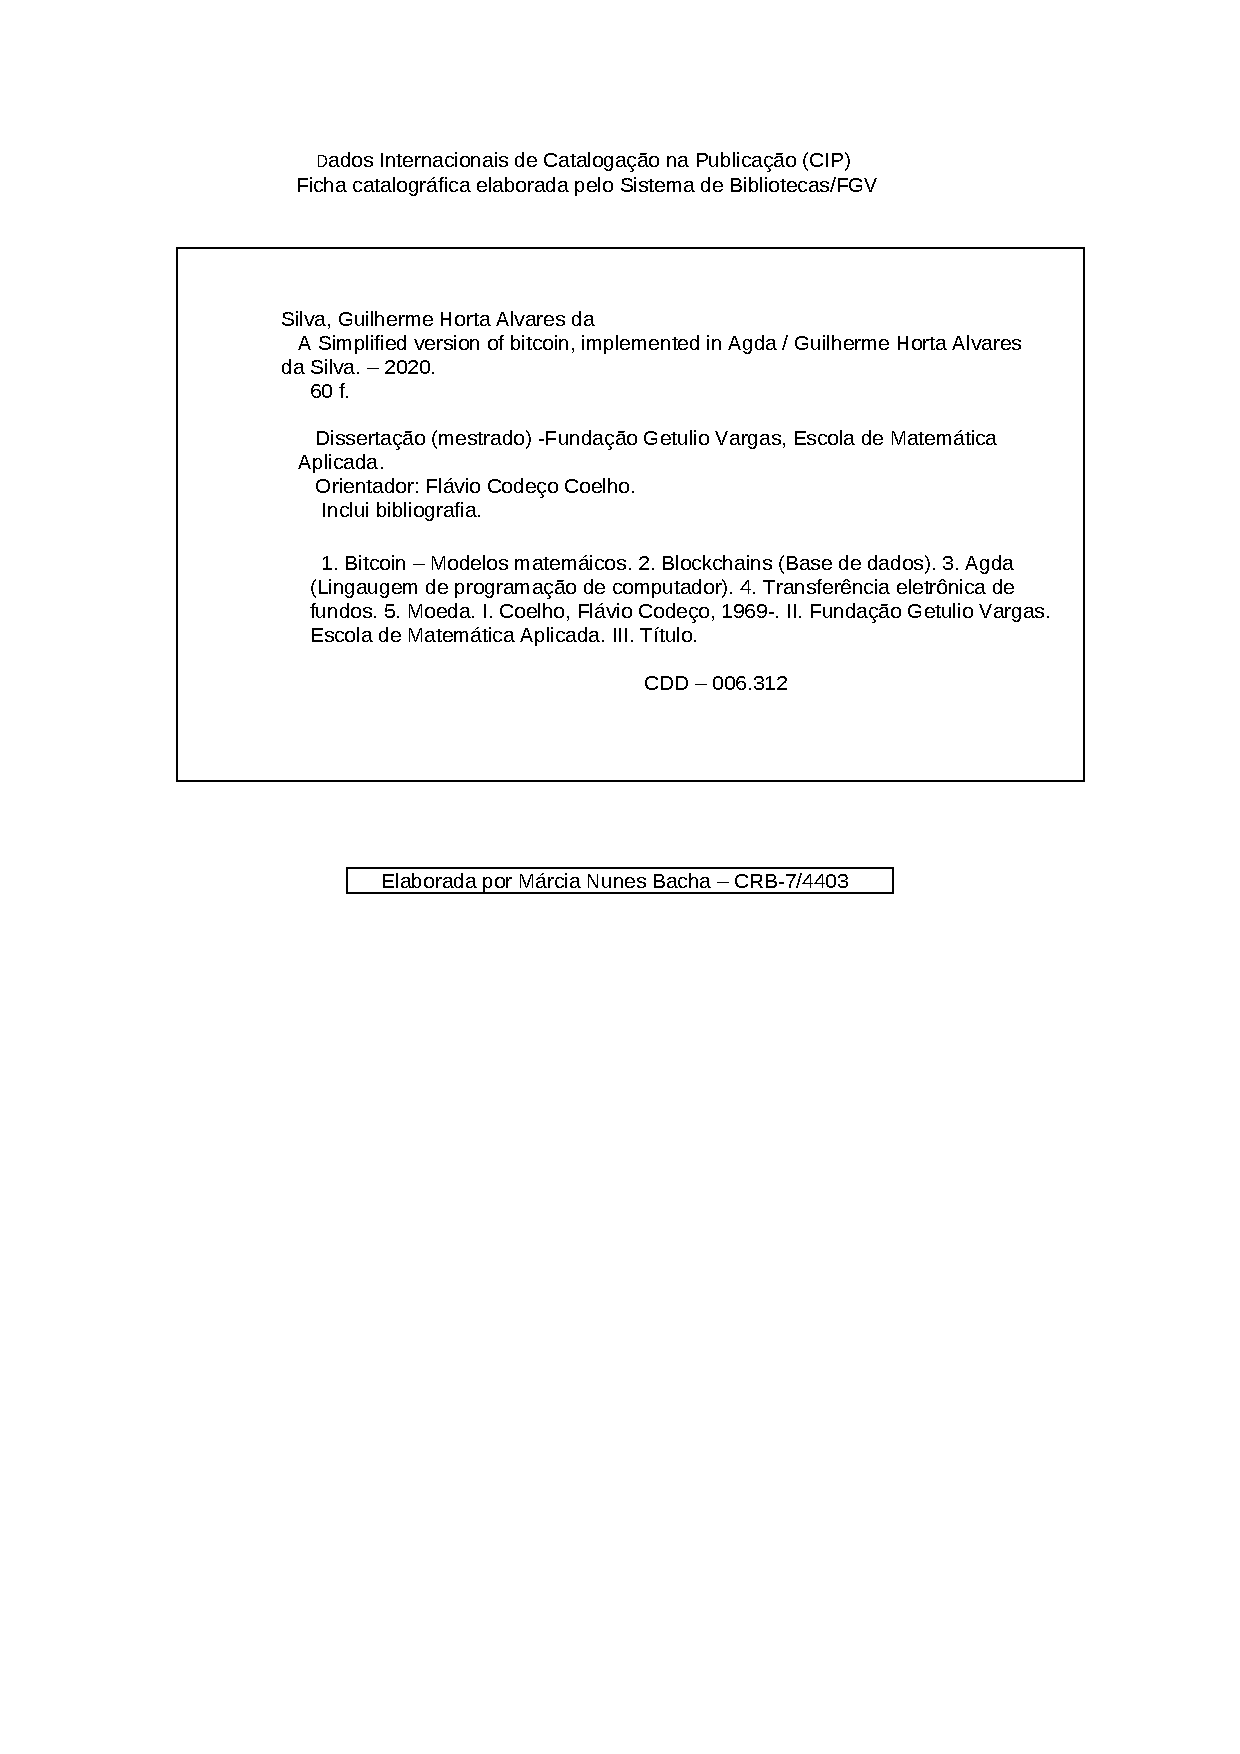
\includepdf[pages=-, offset=75 -75]{ficha.pdf}
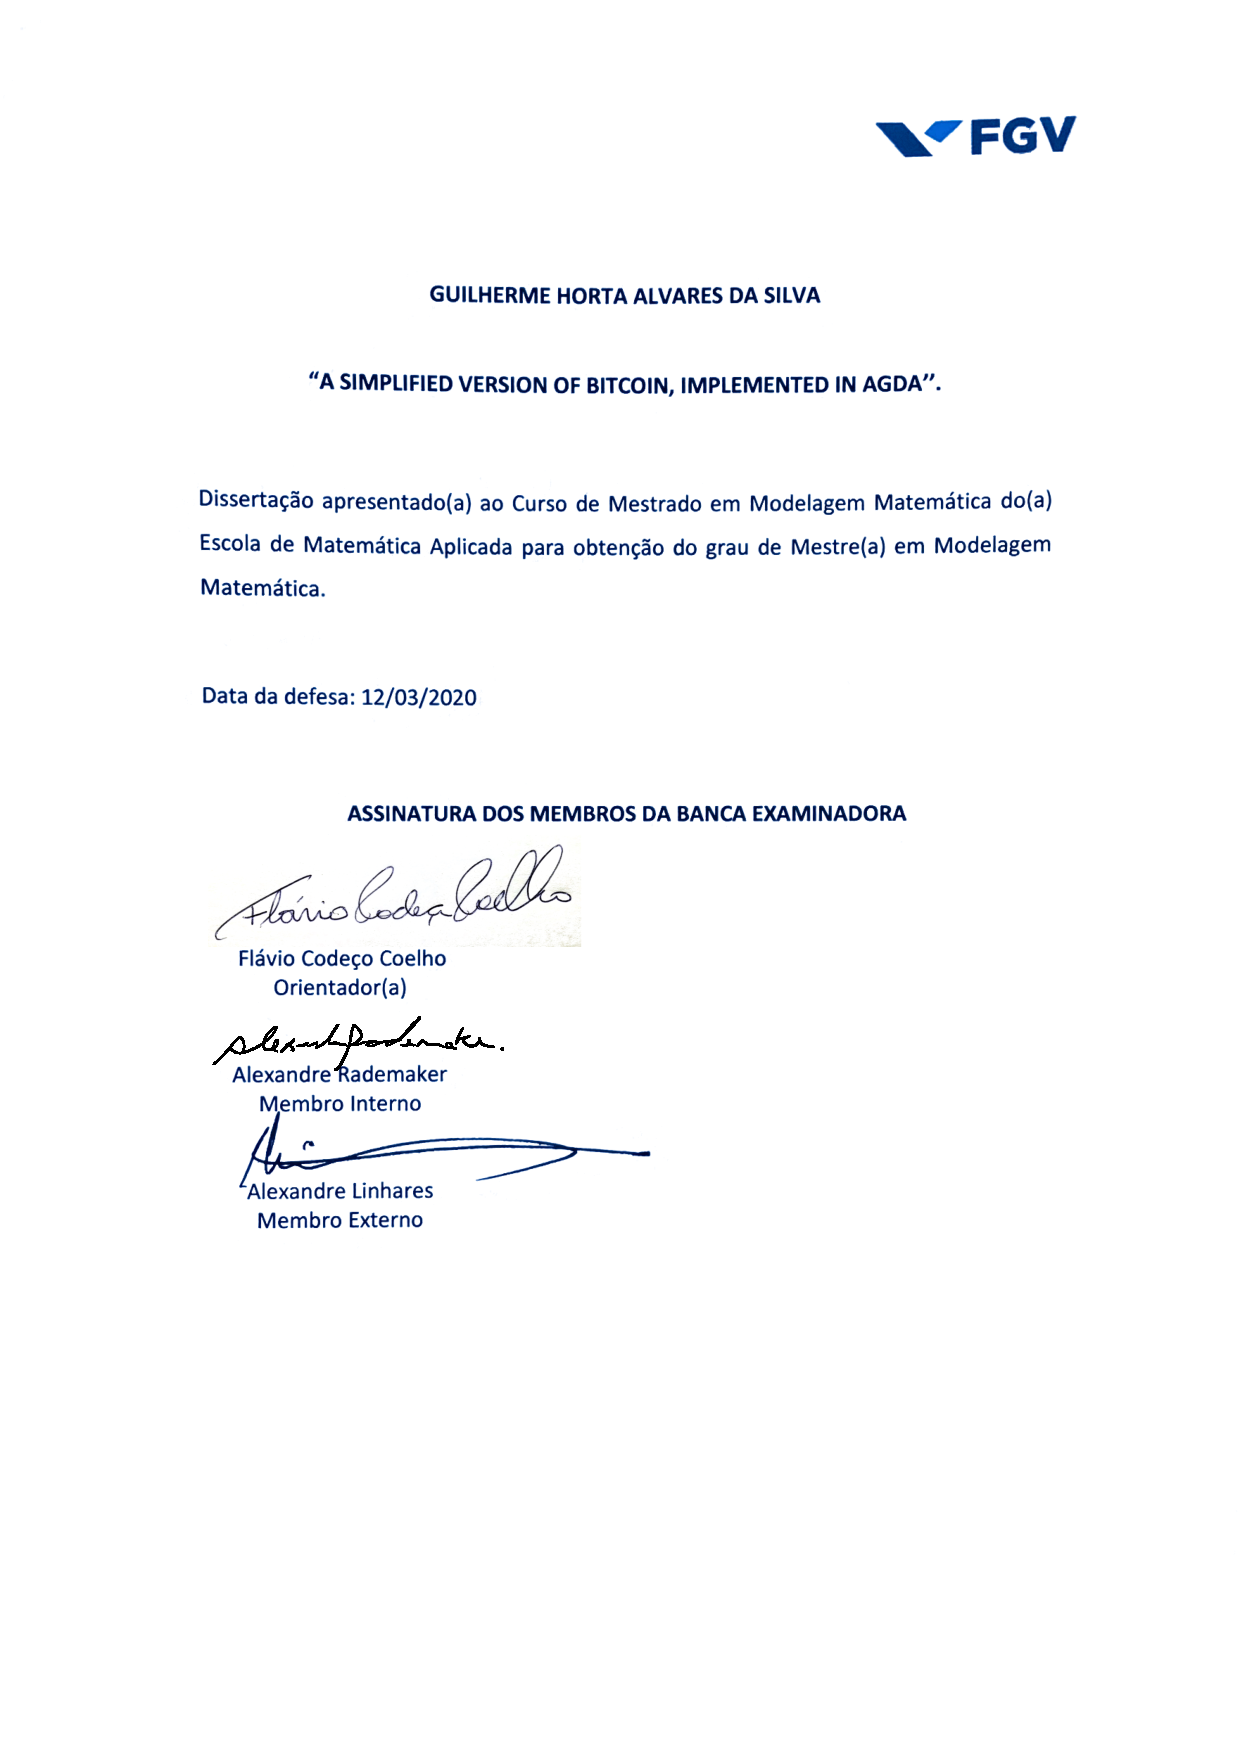
\includepdf[pages=-, offset=75 -75]{assinaturas.pdf}

\section{Abstract}

We present in this work an explanation about what is cryptocurrencies and their principal characteristics,
a brief explanation about Lambda Calculus, dependents types and Agda,
and we present a cryptocurrency model made in this language.
Most of all parts of Bitcoin are coded and typed in this model.
Since transactions, transactions tree, ledger, block, and blockchain.
Cryptographic functions are all postulated like hash functions,
transformation functions of a private key into a public key and addresses.
Besides, in this work, there is code that transforms and validates transactions
from plain text into our model.

\section{Resumo}

Apresentamos nesse trabalho uma explicação sobre o que são criptomoedas e suas principais características,
uma breve explicação sobre o Lambda Calculus, tipos de dependentes e Agda,
e apresentamos um modelo de criptomoeda feito nessa linguagem.
A maioria das partes do Bitcoin é codificada e programada nesse modelo.
Desde transações, árvore de transações, \emph{Ledger}, bloco e cadeia de blocos.
As funções criptográficas, como funções hash,
funções de transformação de uma chave privada em uma chave pública e seus endereços,
são postuladas.
Além disso, neste trabalho, há código que transforma e valida transações
de um texto sem formatação para o nosso modelo.


\subtitle{Acknowledgment}

I would like to give thanks to all the people that helped me in this work.

Thanks, Philip Wadler,
for taught me about programming language foundations and how to code in Agda.
Thanks, Alexandre Rademaker for teaching me the basics of Logic in Lean
and the type theory for the Lambda Calculus in this thesis.
Thanks, Flávio Coelho for being my advisor, for teaching me what Bitcoin is
and helping me writing my dissertation.
In the last, thanks Thais Horta (my mother) for helping me writing better English
and fixing my grammar mistakes.


\printnoidxglossaries
\pagebreak

\listoffigures
\pagebreak

\tableofcontents
\pagebreak

%%%%%%%%%%%%%%%%%%%%%%%%%%%%%%%%%%%%%%%%%%%%%%%%%%%%%%%%%%%%%%%%%%%%%%%%%%%%%%%%%%%%%%%%%
\renewcommand{\thesection}{\arabic{section}}

\section{Introduction}

\subsection{Context} 

In 1983, David Chaum created ecash \cite{panurach1996money} an anonymous cryptographic eletronic money.
This cryptocurrency use \gls{rsa} blind signatures \cite{chaum1983blind} to spend transactions.
Later, in 1989, David Chaum found an electronic money corporation called DigiCash Inc.
It was declared bankruptcy in 1998.

Adam Back developed a \gls{pow} scheme for spam control, Hashcash \cite{back2002hashcash}.
To send an email, the hash of the content of this email plus a nonce has to have a numerical value
smaller than a defined target.
So, to create a valid email, the sender (miner) has to spend a considerable \gls{cpu} resource on it.
Because hash functions produce practically random values, so the miner has to guess a lot of nonce
values before finding some nonce that makes the hash of the email less than the target value.
This idea is used in Bitcoin proof of work because each block has a nonce guessed by the miner and
the hash of the block has to be less than the target value.

Wei Dai propose b-money \cite{dai1998b} for the first proposal for distributed digital scarcity.
And Hal Finney created Bit Gold \cite{wallace2011rise}, a reusable proof of work for hash cash for
its algorithm of proof of work.

On 31 October 2008, Satoshi Nakamoto registered the website ``bitcoin.org'' and put a link for his
paper \cite{nakamoto2008bitcoin} in a cryptography mailing list.
In January 2009, Nakamoto released the Bitcoin software as an open-source code.
The identity of Satoshi Nakamoto is still unknown.
Since that time, the total market of Bitcoin came to 330 billion dollars in 17 of December of 2018
when its value reached a historic peak of 20 thousand dollars.

Other cryptocurrencies like Ethereum \cite{wood2014ethereum}, Monero \cite{noether2015ring} and
ZCash \cite{hopwood2016zcash} were created after Bitcoin,
but Bitcoin is still the cryptocurrency with the biggest market value.

Ethereum is a cryptocurrency that uses an account model instead of \gls{utxo} used in Bitcoin for its
transaction data structure.
It uses Solidity as its programming language for smart contracts which resembles Javascript,
so it is easier to program in it than in the stack machine programming language of Bitcoin.
Ethereum is now transitioning from proof of work (used in Bitcoin) to proof of stake
which will be the default proof mechanism of Ethereum 2.0 and will be released in
3 of January of 2020.

Monero and ZCash are both cryptocurrencies that focus on fungibility, privacy and decentralization.
Monero uses an obfuscated public ledger, so anyone can send transactions,
but nobody can tell the source, amount or destination.
Zcash uses the concept of zero-knowledge proof called \gls{kzsnark},
which guarantee privacy for its users.

\section{Relevant Background}

\subsection{Agda Introduction}
Agda is a dependently typed functional language developed by Norell at the Chalmers University of Technology
as his Ph.D. Thesis.
The current version of Agda is Agda 2.

  \subsubsection{Syntax}
  In Agda, \emph{Set} is equal to type.
  In languages with dependent types, it is possible to create a function that returns a type.

  \agda{agdaExamples}{funcType}

  After the function name, it is two colons (\emph{:}) and the arguments of the function.
  It is closed by \emph{(name\_of\_argument : type\_of\_argument)}.
  After all, there is one arrow and the type of the result of the function.
  This ``if, then, else'' is not a function built-in in Agda.
  It is a function defined this way \emph{if\_then\_else\_} .

  So it is possible to use this function in the default way.

  \agda{agdaExamples}{funcTypeUnd}

  Or use the arguments inside the underscore.

  \agda{agdaExamples}{funcType2}

  The same notation can be done using just arrows without naming the arguments.

  Because of dependent types, it is possible to have a type that depends on the input.

  \agda{agdaExamples}{dependentType}

  It is possible in Agda to do the pattern match.
  So it breaks the input in cases.

  \agda{agdaExamples}{patternMatch}

  To create a new type with a different pattern match, it is used the data constructor.

  \agda{agdaExamples}{dataConstructor}

  This is another example of \emph{Data Set}, but it depends on the argument.

  \agda{agdaExamples}{vector}

  \emph{Vector zero} is a type of a vector of size zero, so the only option to construct it is the empty vector.
  It is constructed from the first constructor.
  Other types of vectors like \emph{Vector 1} (vector of size one), \emph{Vector 2}, ... can only be constructed by
  the second constructor.
  It takes as argument a natural number and a vector and returns a vector with the size of the last vector
  plus one.

  Records are data types with just one case of pattern match.

  \agda{agdaExamples}{record}

  The constructor is the name of the data constructor.

  \hyperref[id]{Implicit terms} are elements that the compiler is smart enough to deduce it.
  So it is not necessary to put it as an argument of the function.

  \plabel{id}
  \agda{agdaExamples}{id}

  Implicit arguments are inside \emph{\{\}}.
  In this example, the name of the Set (\emph{A}) can not be omitted
  (like the second function version of boolean to set),
  because it is used to say that \emph{x} is of type \emph{A}.

  In the case of the function \emph{id}, the type of input can be deduced by the compiler.
  For example, \emph{id} function should be a function from Natural to Natural because
  \emph{zeroN} is already of type Natural.
  In this example, the compiler could figure out the term \emph{A} (Natural) of type \emph{Set}.

  \agda{agdaExamples}{idNat}

  Functions in Agda can be defined in two ways

  \agda{agdaExamples}{funcs}

  In the first case, the arguments are before equal sign (\emph{=}).
  In the second case, it is used the lambda abstraction that means the same thing.

  \agda{agdaExamples}{caseOf}

  \agda{agdaExamples}{filter}

  Filter is a function that filters all elements that have some property already defined.
  In this definition of filter, the lambda abstraction can pattern match
  in the two possibilities of \emph{p x}, that are \emph{true} or \emph{false}

  \agda{agdaExamples}{filterWith}

  The \emph{with} abstraction is the same thing as the \emph{case of}.
  Before the \emph{=}, there are the possibilities of \emph{p x} (\emph{true} or \emph{false}).

  \agda{agdaExamples}{postulate}

  In Agda, the \emph{postulate} assumes that there is one element of a given type without defining it.
  In this example, \emph{someBot} is an element of the empty type.
  Postulate can be dangerous because it assumes that some element of a given type exists,
  but it can not (like in the example).

  \agda{agdaExamples}{rewrite}

  In Agda, \emph{rewrite} means changing the returned type of the result.
  Because $a + b ≡ b + a$, returning an element of the type $P (a + b)$ is the
  same thing that returning an element of the type $P (b + a)$.

  \subsubsection{Lambda Calculus}
  Lambda Calculus is a minimalist Turing complete programming language with the concept of abstraction,
  application using binding and substitution. For example, \emph{x} is a variable, $(\lambda x.M)$
  is an Abstraction and (\emph{M N}) is an Application.

  In Lambda Calculus, there are two types of computational conversions $\alpha$-conversion
  and $\beta$-reduction.
  In $\alpha$-conversion, $(\lambda x.M[x]) \rightarrow (\lambda y.M[y])$.
  So in every free variable \emph{x} in \emph{M} will be renamed to \emph{y}.
  For \emph{M[x] = x}, an $\alpha$-conversion is $(\lambda x.x) \rightarrow (\lambda y.y)$

  A free variable is every variable that is not bound outside.
  For example, $((\lambda\textcolor{green}{x}.\textcolor{blue}{x}) \textcolor{red}{x})$.
  The \textcolor{blue}{blue x} is bonded for the \textcolor{green}{green x},
  but the \textcolor{red}{red x}
  is not bonded for any function. So the \textcolor{red}{red x} is a free variable.

  In $\beta$-reduction, it replaces the all free for the expression in the application.
  The $\beta$-reduction of this expression $((\lambda x.M) N) \rightarrow (M[x := N])$ .
  So if $M = x$, the $\beta$-reduction will be $((\lambda x.x) N) \rightarrow N$.
  If $M = (\lambda x.x) x$, the $\beta$-reduction will be
  $(\lambda x.((\lambda x.x)x))N \rightarrow (\lambda x.x)N$.

  Agda uses typed lambda calculus.
  So in an application \emph{(M N)}, \emph{M} has to be of type $A \Rightarrow B$ and N has to be of type A.
  $(\lambda (x : A) . x)$ is of type $A \Rightarrow A$, because \emph{x} is of type \emph{A}.

  \agda{lambdaCalculus}{Id}
  The simplest function is the identity function made in Agda.

  \plabel{id2}
  \agda{lambdaCalculus}{Id2}
  \hyperref[id2]{This} is another way of writing the same function.

  \plabel{truefalse}
  \agda{lambdaCalculus}{trueFalse}
  \hyperref[truefalse]{This} is how true and false are encoded in lambda calculus.

  \plabel{naturals}
  \agda{lambdaCalculus}{naturals}
  \hyperref[naturals]{This} is how naturals numbers are defined in lambda calculus.
  Look that the definition of zero looks like the definition of false.

  \agda{lambdaCalculus}{isZero}
  Defining natural numbers in this way, it is possible to say if a natural number is zero or not.

  \agda{lambdaCalculus}{plus}
  Plus is defined this way using lambda calculus.

  \plabel{onepone}
  \agda{lambdaCalculus}{onePone}
  \hyperref[onepone]{This} is one example of the calculation of one plus one in Lambda Calculus.

  \plabel{list}
  \agda{lambdaCalculus}{list}
  \hyperref[list]{This} is how lists are defined in Lambda Calculus.

  \agda{lambdaCalculus}{sumList}
  Substituting the cons operation of list per plus and nil list to zero, it is possible to calculate
  the sum of the list.

  \agda{lambdaCalculus}{either}
  In this way, it is possible to define \emph{Either}.
  It is one way to create a type that can be a Natural or a Boolean.

  \agda{lambdaCalculus}{eitherExamples}
  In these examples, it is defined zero, one in left and false, true in right.

  \agda{lambdaCalculus}{eitherRes}
  \emph{Either} is useful when defining one function that works for left and another that works for the right.
  If the natural number is zero, the function chosen is the left and
  if it is an identity, the function chosen is the right. 

  \plabel{tuple}
  \agda{lambdaCalculus}{tuple}
  \hyperref[tuple]{This way} is how tuple is defined in Lambda Calculus.

  \plabel{tupleexamples}
  \agda{lambdaCalculus}{tupleExamples}
  \hyperref[tupleexamples]{This} is how is defined the tuple zero false and the tuple one true.

  \plabel{tupleadd}
  \agda{lambdaCalculus}{tupleAdd}
  \hyperref[tupleadd]{This} is one way of defining a function that adds one to the argument
  if the first element of the tuple is true.


  \subsubsection{Martin-Löf Type Theory}
  Agda also provides proof assistants based on the intentional Martin-Löf type theory.

    In Martin-Löf type theory, there are three finite types and five constructors types.
    The zero type contains zero terms. It is called the empty type and it is written $\bot$.
    \agda{agdaExamples}{botType}

    The first type is the type with just one canonical term and it represents existence.
    It is called unit type and it is written top.
    \agda{agdaExamples}{trivialType}

    The second type contains two canonical terms. It represents a choice between two values.
    \agda{agdaExamples}{eitherType}

    The Boolean type is defined using the Trivial type and the Either type.
    \agda{agdaExamples}{boolType}

    If statement is defined using booleans.
    \agda{agdaExamples}{ifThenElse}


    \subsubsection{Types Constructors}
    The product-types contain an ordered pair.
    The second type can depend on the first type.
    \agda{agdaExamples}{mulType}

    \agda{agdaExamples}{mulEx}
    In the function $\exists-vec$, the product-type has the same meaning of exists.
    This type means that
    ``Exists a natural number \emph{n} that there is one element of type \emph{Vector A n}''

    The $\pi$-types contain functions.
    So given an input type, it will return an output type.
    It has the same meaning as a function:
    \agda{agdaExamples}{piType}

    In Inductive types, it is a self-referential type.
    Naturals numbers are examples of that:
    \agda{agdaExamples}{Nat}
    Other data structures like a linked list of natural numbers, trees, graphs are inductive types too.

    Proofs in inductive types are made by induction.
    \agda{agdaExamples}{NatElim}

    Universe types are created to allow proofs written in all types.
    For example, the type of \emph{Nat} is \emph{U0}.


Agda has dependent types like in CoQ but does not have tactics.
Agda is a total language, so it is guaranteed that the code always finish
(impossible infinite loops) and coverage all inputs.

Agda has inductive data types that are similar to algebraic data types in non-dependently
typed programming languages.
The definition of Peano numbers in Agda is:

\agda{agdaExamples}{Nat}

Definitions in Agda are done using induction.
For example, the sum of two numbers in Agda:

\agda{agdaExamples}{sum}

In Agda, because of dependent types, it is possible to make more expressive types that are not
possible in other languages.
For example, get the first element of a vector.
For it, it is necessary to specify in the type that the vector should have a size greater than zero.

\agda{agdaExamples}{vecHead}

Another good example is that in the sum of two matrices, they should have the same dimensions.

\agda{agdaExamples}{matrixSum}

\subsubsection{Preposition as Types}

In Agda, types can be seen as prepositions and terms of this given type like a proof.
For example, \emph{x} can be a term of the type \emph{A}.
So \emph{x} is a proof that \emph{A} holds.

\agda{agdaExamples}{id}

In the function \emph{id},
if there is a proof \emph{x} that \emph{A} holds,
so \emph{A} holds.
The function \emph{id} is a proof of $A \rightarrow A$.

\agda{agdaExamples}{and}

In the function \emph{and}, \emph{a} is a proof that \emph{A} holds and
\emph{b} is a proof that \emph{B} holds,
so \emph{a , b} is a proof of $A \times B$

\agda{agdaExamples}{equality}

Equality function can be seen as
``For all elements of \emph{x} in the Set \emph{A}, $x \equiv x$''.
If there is a term of this type, so this preposition is true.
In this case, the term is a function that given a term \emph{x} of type \emph{A},
it returns \emph{refl \{\_\} \{\_\} \{x\}}.
\emph{refl} is a constructor of equality, so \emph{refl \{\_\} \{\_\} \{x\}}
returns a term of type $x \equiv x$.

\subsection{Bitcoin Overview}

The Bitcoin was made to be a peer to peer electronic cash.
It was made in one way that users can save and verify transactions without the need of a trusted party.
Because of that no authority or government can shut down the Bitcoin.

\incimg{transactions1}{png}{Transaction}
%% https://medium.com/coinmonks/bitcoin-transactions-be401b48afe6

Transactions in Bitcoins (like in \figref{transactions1}) are an array of input of
previous transactions and an array of outputs.
Each input and output is an address, each address is made from a public key
that is made from a private key.

\incimg{privatekey}{png}{Bitcoin account}
%% https://coinsutra.com/bitcoin-private-key/

A private key is a big number.
It is so big that it is almost impossible to generate two identical private keys.

The public key is generated from the private key
(like in \figref{privatekey} where the account number is f(p)),
but a private key can not be generated from a public key.

In Bitcoin, the miner is someone that calculates a value \emph{nounce} for each block.
Because of that, he receives all transaction fees of this block plus a block reward.
The mining transaction (made for the miner) does require an input.
For each input transaction, it is necessary a signature signed with a private key
(like in \figref{privatekey} where the signature is f(p,t))
to prove the ownership of the Bitcoins.
With the message and the signature, it is possible to know that the owner of the private key
that generates the public key signed the message.

Signature is created from a function that receives as inputs the private key and the message.
There is no analytical form of the inverse of this function.
Because of that, the only way of finding an element \emph{x} that this function \emph{f} so
that $f(x) = y$ for a given \emph{y} is trying for random different values of \emph{x}.
So it is almost impossible to find the private key from a message, a signature, and the public key.
In \figref{privatekey}, the checker is a f(t,s,a).
So because of that, the owner of the private key can sign several messages without anyone knows
his private key.

\incimg{transactions2}{jpg}{Verification and signature of transactions}
%% https://en.wikipedia.org/wiki/Bitcoin_network

Transactions (shown in \figref{transactions2}) are grouped in a block (shown in \figref{blockchain}).
Each block contains in its header the timestamp of its creation, the hash of the block,
the previous hash and a nonce.
A nonce is an arbitrary value that the miner has to choose to make the hash of the block respect some
specific characteristics.

\incimg{blockchain}{png}{Blockchain}
%% https://bitcoin.stackexchange.com/questions/12427/can-someone-explain-how-the-bitcoin-blockchain-works/13347
%% https://i.stack.imgur.com/HrKX0.png

Each block has a size limit of 1 MB.
Because of that, Bitcoin forms a blockchain (a chain of blocks).
Each block should be created at an average of 10 minutes.
The advantage of using a short average time of block creation is that it will propagate transactions
faster in the blockchain.
But the disadvantage is that it increases the probability of creating orphan blocks.
To make the blockchain tamper-proof (nobody can alter an existing block),
there is a concept called proof of work in Bitcoin.
To create a new block, the creator (called the miner) has to choose a random value as nonce that makes
the hash of the block less than a certain value.
This value is chosen in a way that each block should be generated on 10 minutes on average.
If the value is for example 100 and the total possibilities of results are 10.000 (codomain),
the probability of finding \emph{x} so that $hash(x) \leqslant 100$ is 1\% $100/10.000$.
Because of that, in this example, the miner has to calculate on average 100 hashes before finding
the right one.

If the value is too low, miners will take more time to find a nonce that makes the hash block
less than it.
If it is too high, it will be easier to find a nonce and they will find it faster.

When two different blocks are created in nearly the same time, there are two valid blockchains.
It is because the last block in both blockchains are valid but different.
Because of this problem, in the Bitcoin protocol, the largest chain is always the right chain.
While two valid chains have the same size, it is not possible to know which chain is the right.
This situation is called fork and when it happens, it is necessary to wait to see in which chain
the new block will be.

If miners have more than 50\% of the hash rates of Bitcoin, they can do an attack called a
51\% attack.
It happens when some miner, with more power than all network, mine secretly the blocks.
So if the main network has 50 blocks, the miner could produce hidden blocks from 46 to 55
and he would have 10 hidden blocks from the network.
When he shows their hidden blocks, his chain becomes the valid chain, because it is bigger.
So all transactions from the previous blockchain from 46 to 50 blocks become invalid.
Because of that, when someone makes a big transaction in the blockchain, it is a good idea
to wait more time.
So it is becoming harder and harder to make a 51\% with more time.
Bitcoin has the highest market value nowadays, so attacking the Bitcoin network is very expensive.
Nowadays, this kind of attack is more common in new altcoins.

Ledger is a software that tracks how much money each address can spend.
It can be known when calculating the sum amount of all unspent output transactions destined
for each address.

The \gls{utxo} model used in Bitcoin and the account model used in Ethereum are the two most used kinds
of data structures to model account records and savings states.

In the account model, it is saved the address and the balance of each address.
For example, the data structure will look like this [(0xabc01, 1.01), (0xabc02, 2.02)].
So the address 0xabc01 has 1.01a of balance and the address 0xabc02 has 2.02 of balance.
In this way, it is possible to easily know how much balance each address has,
but it is not possible to know how they got in this state.

  \incimg{utxo}{png}{UTXO transactions}
  %% https://bitcoin.org/
  %% https://medium.com/@sunflora98/utxo-vs-account-balance-model-5e6470f4e0cf

In the \gls{utxo} model (shown in \figref{utxo}), each transaction is saved in the transaction tree.
Every transaction is composed of multiples inputs and multiples outputs.
But all inputs have to come from outputs that have never been spent before.

Because of that, in the \gls{utxo} model, it is easy to make a new transaction from the previous one,
but it is harder to know how much each one has.
To know how much someone has, it is necessary to calculate the sum of all unspent transaction outputs
destined for his addresses.

In the account model, there could be one kind of vulnerability
that is less probable to happen in the \gls{utxo} model.
Changing both addresses balances is not an atomic operation.
Because there are two instructions, subtracting the balance of the sender
and incrementing the balance of the receiver.
If something bad happens between these two instructions, the final state
will become an invalid state.

For example: \\
\textbf{
bobBalance -= 1 \\
Intermediary State \\
aliceBalance += 1
}

In the account model, it is straight forward to know how much balance each address has.
In the \gls{utxo} model, this calculation is made off-chain. It can be a good thing
because each user has more privacy.

\subsection{Ethereum}

Ethereum differs from Bitcoin in having an \gls{evm} to run script code.
\gls{evm} is a stack machine and Turing complete \cite{turing1936computable} while Bitcoin Script is not
(it is impossible to do loops and recursion in Bitcoin).

Transactions in Bitcoin are all stored in the blockchain.
In Ethereum, just the hash of it is stored in it.
So it is saved in the off-chain database.
Because of that, it is possible to save more information in Ethereum Blockchain.

Contracts in the blockchain are the script program that comes with the transaction.
In Bitcoin, the creator of the contract has to pay the amount proportional to its size.
In Ethereum, it is different.
Each smart contract in Ethereum is made by a series of instructions.
Each instruction consumes different the computational effort.
Because of that, in Ethereum, there is a concept of gas, that measure how much computational effort
each instruction needs.
So in each smart contract, it is well know how much computational effort will be necessary to run it
and it is measured in gas.
Because computational effort of each node in the Ethereum network is a scarce resource,
to execute the smart contract, it is necessary to
pay an amount in ether for each gas to the miner run it.
Smart contracts that pay more ether per gas run first because the miner will want to have the best
profit and they will pick them.
If the amount of ether per gas paid is not high enough, the contract will not be executed,
because some other contracts pay more that will be executed instead of this one.

Because Ethereum has its \gls{evm} with more instructions than Bitcoin and it is Turing Complete,
it is considered less secure.
Ethereum has its high-level programming language called Solidity that looks like JavaScript.


\section{Development}
  \subsection{Crypto Functions}
The first thing that we define is the crypto functions that will be needed to make the cryptocurrency.
Messages can be defined in multiple ways, one array of bytes, one string or a natural number.
Messages in this context means some data.

The private key is a number, a secret that someone has.
In Bitcoin, the private key is a 256-bit number.
A private key is used to signed messages.

The public key is generated from a private key.
But getting the private key from a public key is really difficult.
To verify who signed a message with a private key, he has to show the public key.

Hash is an injection function (the probability of two functions having the same hash is very low).
The function is used from a big domain to a small domain.
For example, a hash of big file (some GBs) is an integer of just some bytes.
It is very useful to prove for example that 2 files are equal.
If the hash of two files are equal, the probability of these files being equal is really high.
It is used in torrents clients, so it is safe to download a program to untrusted peers,
just have to verify if the hash of the file is equal to the hash of the file wanted.

These functions can be defined, but it is not the purpose of this thesis.
So they will be just postulates.

\agda{Crypto}{cryptoPostulates}

  \subsection{Transactions}

\subsubsection{Definitions}

In Bitcoin, there are some transactions.
In each transaction, there are multiple inputs and outputs.
Each input is named TXFieldWithId.
The input of one transaction is the output of another transaction.
Firsts outputs are generated from coinbase transaction (created by the miner).
Each block has just one of this transaction.

\agda{Transactions}{VectorOutput}

Vector output is the vector of outputs transactions.
It is a non-empty vector, because it already starts with one element \emph{fstStart}
or it is an union from one transaction with another vector.
In its representation, it is possible to know in what time it was created (time is the position of
they in all transactions),
what is his size (quantity of outputs fields)
and the total amount spent in this transaction,

\emph{elStart} is a proof that the position of TXFieldWithId is the last one,
because its position in the vector is the same as the last position (size) of the vector.
It is used after to specify which input is in the transaction.

\agda{Transactions}{TXSigned}

A signed transaction is composed of a non-empty list of inputs and outputs.
For each input, there is a signature that confirms that he accepted every output in the list of outputs.
And in the transaction, there is proof ($in \geq out$) that the total amount of money
in all inputs are bigger than the total amount of outputs.
The remainder will be used by the miner.

\subsubsection{Raw Transaction}

Raw transactions are transactions without any explicit dependent type.
Here the definition of \emph{raw signed transaction}:

\agda{RawTransactions}{rawtxsigned}

\emph{Raw signed transactions} is a record with \emph{inputs}, \emph{outputs}
and the signature of \emph{inputs} and \emph{outputs}.

The definition of some important types:

\agda{Crypto}{cryptoTypes}

The definition of \emph{Raw Input}:

\agda{RawTransactions}{rawinput}

In each input, it is necessary to know the time, the position of it in the transaction,
the amount spent, its message, the signature, and its public key.
The signature is the signature of the message.
And the message is usually related to the amount spent in each output.

The definition of \emph{raw transaction}:

\agda{RawTransactions}{rawTransaction}

It is all inputs and all outputs.

The definition of \emph{Raw TX}:

\agda{RawTransactions}{rawTX}

The definition of \emph{raw transaction coinbase}:

\agda{RawTransactions}{rawCoinbase}

The defintion of \emph{raw Vector Output}: 

\agda{RawTransactions}{rawVecOut}

It has the time, its size, the total amount, the \emph{vector output}
and proof that this vector is the same as the list of outputs of this type.

The definition of the record that every input transaction is signed in a given time:

\agda{RawTransactions}{txsigall}

It has the size of vector output, the sublist of all inputs, the total amount,
the \emph{vector output} and a proof that all sublist of inputs are signed.

$rawTXSigned \to TXSigAll$ returns a signed transaction of all inputs in a given time
if \emph{rawTXSigned} has valid signatures for all these inputs:

\agda{RawTransactions}{rawtxSigToTxsigAll}

It has to validate first that the \emph{list of outputs} is a valid \emph{Vector Output}.
Second, it validates if the signature of the inputs are valid with the
\emph{raw signed transaction}.
In the last case, it validates if the time of the \emph{vector output} is equal
of the time of this transaction.
If all conditions match, it returns a proven signed transaction.
If not, it returns nothing.

\hyperref[rawToTX]{This function} transforms a \emph{raw transaction} into a \emph{signed transaction}:

\plabel{rawToTX}
\agda{RawTransactions}{txrawToTxsig}

The function $vecOut \equiv ListAmount$ returns a proof that the \emph{vector output} is equal
to the total amount of the \emph{list of transactions}.
It is impossible that the \emph{vector output} is equal to an empty list.
In case that the list has just one element, it just has to return \emph{refl}.
The another case, it is done recursively.

The proof that the amount of input transaction is greater than the amount of output
is just a rewrite from the previous proof ($vecOut≡ListAmount outputs vecOut out≡vec$).

The function \emph{sameMessage} returns a proof that the message of \emph{raw transaction}
is the same as the message of the \emph{vector output}.
In case that \emph{vector output} has just size one or two, it is a trivial case.
The other cases are doing it recursively.

\emph{sigPub} is another function that returns a proof that an input message is signed.
It validates it with its public key.

The last function returns a proof that every input was signed.
It is done in a recursive way using the function \emph{sigPub}.

This is the function that transforms a list ot transactions into a possible \emph{vector output}:

\agda{RawTransactions}{listTXFieldtoVecOut}

The list has to be at least with a size one.
Because the \emph{vector output} can not be empty.
To add one element into the vector, it has to verify if the time is equal to the first time.
Another verification is that the informed position in the vector is right.
If all validations are right, it returns the vector output.
If it is not, it returns nothing.

The definition of the function that transform a \emph{raw transaction} into a
\emph{raw signed transaction}:

\agda{RawTransactions}{rawtoTXSigned}

The first validation that the function does is verifying that the outputs are not empty.
Another validation is verifying if the amount spent on inputs is greater than the amount of the outputs.
The function \emph{Signed?}, defined in the crypto library, validates if the
message was signed with the input.
After, it validates if all inputs are signed.
If all validations are right, it returns the \emph{raw transaction signed}.
If it is not, it returns nothing.

  \section{Transaction Tree}

\subsection{Definition}

The transaction tree is one of the most important data structures in Bitcoin.
In the transaction tree, there are all unspent transaction outputs (UTXO).
In every new transaction, the UTXOs used as input is removed from the transaction tree.

\agda{TXTree}{TXTree}

In this implementation, time is the number of transactions in TXTree.
Block is related to which block the transaction tree is.
After every new coinbase transaction (the miner transaction), the block size increment in one quantity.
Total fees are how much the miner will have in fee of transactions if he makes a block with these
transactions.
Quantity of transactions is how many transactions there are in the current block.
The type is tQtTxs instead of a natural number because, in this implementation, each block can have
a number maximum of transactions.
In Bitcoin, it is different, each block has a limit size in space of 1 MB.

Genesis tree is the first case.
It is when the cryptocurrency was created.
\emph{txtree} is created from another tree.
\emph{proofLessQtTX} is proof that the last transaction tree has its
block size less than the maximum block size minus one or it is a coinbase transaction.
It is because it is necessary to verify the size of the last \emph{txtree} so it will not have
the size greater than the maximum.

\agda{TXTree}{TX}

TX is related to the transaction done in the cryptocurrency.
There are two kinds of transaction.
Coinbase transaction is the transaction done by the miner.
In coinbase, they have just outputs and do not have any input.
\emph{pAmountFee} is proof that the output of the coinbase transaction is equal to the total fees plus
a block reward.

Another kind of transaction is the \emph{normalTX}, a regular transaction.
\emph{SubInputs} are a sub-list of all unspent transaction outputs of the previous transaction tree.
Outputs are the new unspent transaction from this transaction.
So who receives the amount from this transaction can spend it after.
\emph{TxSigned} is the signature that proves that every owner of each input approve this transaction.
In \emph{TxSigned}, there is proof that the output amount is greater than the input amount too.

\agda{TXTree}{isCoinBase}

This function just returns trivial type if coinbase and bot type if not.

\agda{TXTree}{nextBlock}

If it is a normal transaction, the block continues the same.
If it is a coinbase transaction, the next transaction will be in a new block.

\agda{TXTree}{incQtTx}

This function is to increment the number of transactions in the block.
It has to receive proof that the quantity of transaction that was before this new transaction was
less than then the maximum quantity of transactions allowed.
So it is guaranteed that the number of transactions will never be greater than the maximum allowed.
If it is a coinbase transaction, it will be a new block.
So the number of transactions starts being zero.

\agda{TXTree}{incFees}

\emph{IncFee} is a function that increments how much fee the miner will receive.
If it is a coinbase transaction, the fee will be received by the miner,
so the next miner will not receive this previous fee.
Because of that, the new fee will start from zero.
If it is a normal transaction, the newest fee will be the amount of input of the transaction minus
the output of this transaction plus the last fee of previous transactions.

\agda{TXTree}{outFee}

\emph{outFee+RewardBlock} is proof that the amount of output transactions is equal to total fees of
other transactions plus the block reward.

\subsection{Raw Transaction Tree}

The raw transaction tree is the tree without the explicit types.
Here, the definition:

\agda{RawTXTree}{rawtxtree}

A good utility of raw data types is that it is not necessary to add type arguments in functions.
Here, a function that adds a transaction to a transaction tree.
If this transaction is compatible with the transaction tree,
it returns a new transaction tree.
If it is not compatible, it returns nothing.
A better solution is a proof that this transaction is invalid with the transaction tree
instead of nothing.
But defining what is an invalid transaction can be tricky.

\agda{RawTXTree}{addtxtree1}

There are two cases.
The first one is if the transaction is a coinbase transaction.
It tries first to transform a list of \emph{TXField} into \emph{VecOut}.
If it can not transforms, it returns nothing.
If it can, it validates if the amount of vector output is equal to total fees plus the block reward.
After, it validates if the time of the transaction is equal to the time of the transaction tree.
In the end, it adds the outputs of the transaction to the vector of outputs.
Because it is a coinbase transaction, there are no inputs to be removed.

\agda{RawTXTree}{addtxtree2}

The second case, that the transaction is regular, looks like the same.
First, it validates if the quantity of transaction is less than the maximum allowed.
Second, it validates if this transactions is a valid signed transaction.
If all these conditions are true, it returns a new transaction tree
with news outputs equal to the outputs of this transaction plus the outputs of the last transaction tree
minus the inputs.
In case of an invalid transaction, it returns nothing.

\subsection{Proofs}

One of the important proofs is that each output of \emph{outputs transaction} is distinct.
This is very important because it guarantees that each input in the transaction could be
just related to just one unspent output.
This characteristic could be in the type of transaction tree,
but it is proven outside of it.

First, it is necessary to define what is a distinct union:

\agda{Utils}{uniondist}

The union of distinct lists makes a new distinct list if both are distinct to each other.

Now, to prove that outputs are a distinct list:

\agda{proofsTXTree}{uniqueouts}

In the first case, the transaction tree is a genesis tree without any outputs.
So an empty list is a distinct list.
In the second case, the outputs are the union of inputs of the transaction with the outputs
of \emph{vector output}.
So, it is necessary to prove that inputs of the transaction are distinct,
that elements of \emph{vector output} are also distinct and that both lists are distinct to each other.

\agda{proofsTXTree}{distinps}

There are some cases to prove that inputs are distinct.
First, if it is a regular transaction or if it is a coinbase transaction.
Second, if the transaction tree of this transaction is a genesis tree or if it is a regular tree.

If the transaction tree of the transaction is a genesis tree,
the number of inputs is zero.
So they are distinct.

In other cases, it does the same thing as proof of unique outputs.
The only difference is that it also does a recursive proof.
It assumes that the transaction of the last transaction tree is also distinct.

\agda{proofsTXTree}{alldists}

Both are distinct to each other because all of the transactions of input has the timeless
then the time of the transaction.
And because all of the outputs of the current transaction has time equal to the current time
of this transaction.

\agda{proofsTXTree}{outtimeless}

The proof that the time of the outputs is less than the current time of the transaction
is done recursively.
It is both necessary to proof that \emph{inputs of tx} and \emph{vector output} have both
times less than the current time of this transaction.
It is all done recursively.

  \subsection{Ledger}

Ledger in the cryptocurrency is like a wallet.
It makes it easier for users to send their coins or to know how much money they have in total.

Here, the definition of how much money the user has in the last tree:

\agda{Ledger}{ledgertree}

The definition of \emph{ledgerOut}:

\agda{Ledger}{ledgerout}

If there is no output, it returns zero of the amount.
If there is at least one output, it verifies if the output address is the same as the address.
If it is, it adds the amount to the amount of the rest of the outputs.
If it is not, it just returns the result of the recursion of the rest of the outputs.

Here, the same code for list of outputs without id:

\agda{Ledger}{ledgernoid}

  \section{Blockchain}

\subsection{Definition}

Block is a chain of transactions that is added in Bitcoin blockchain in every ten minutes.
Each block consists of several transactions and a miner transaction.
This is how a block is defined in this work:

\agda{Blockchain}{block}

\emph{nextTXTree} assures that the second transaction tree is from the first transaction tree.
\emph{firstTreesInBlock} guarantees that the last transaction in the first transaction tree
is the first in the block.
\emph{coinBaseTree} assures that the last transaction in the second transaction tree is
a coinbase transaction.

Blockchain is a chain of valid blocks.
Every new block must be a continuation of the previous one.
Here is the definition of the blockchain:

\agda{Blockchain}{blockchain}

In the first case, blockchain just has one block, called \emph{fstBlock}.
In the second case, the blockchain is an addition of a valid block from a previous blockchain.

\subsection{Creation}

To create a blockchain, it is first needed to create the last block.
From the last block, it is possible to create all the chain.

\agda{Blockchain}{blockblockchain}

In this proof, if the first transaction tree of the block is a genesis tree,
it will return a blockchain of just one block.
If it is a regular tree, it tries to find the first transaction tree of this block.
Using a recursive definition of block to blockchain,
it is possible to generate all the rest of this blockchain from this block.

It is not always possible to generate a block from the transaction tree.
It is because the last transaction of a transaction tree must be a coinbase transaction.
Here, the function that returns a decidable if it is possible to generate a block from
the transaction tree.

\agda{Blockchain}{treeblock}

The definition of the raw block gets just the coinbase transaction tree as an explicit type.
The other transaction tree can be founded opening the record.

\agda{Blockchain}{rawblock}

The code of the definition of what is a coinbase tree:

\agda{Blockchain}{coinbasetree}

The definition of a coinbase tree is the one that the last transaction is a coinbase.

The code verifies if the last transaction tree is a coinbase tree:

\agda{Blockchain}{iscoinbase}

If it is, it returns that it is possible to create a block from that with the block definition.
If it is not, it returns that it is impossible to create a block from this transaction tree.

But to create a block from this coinbase transaction tree, it is necessary to find the first tree
of the block.

\agda{Blockchain}{fsttree}

The definition of \emph{fstTree} is that it has a tree that is before this tree in the type.
And this tree before is the first in the block.

\agda{Blockchain}{firsttreeinblock}

The decidable version of this \emph{Set}:

\agda{Blockchain}{isfirsttreeinblock}

In this case, it pattern match trees that are genesis tree or if the last transaction was a coinbase
transaction.

\agda{Blockchain}{firsttree}

To find the first tree in the block, there are two cases.
The first case is that if the tree is a genesis tree, so the result is itself.
The second case is if it a regular tree, so it still has to divide it in many cases.
If this tree is already the first tree in the block, it will return itself.
If this tree is not, it has to verify if the block number of the tree is the same as this tree.
If the block number is equal, it can recursively find the first tree.
If it is not, it has to provide proof that this tree must be
the first and the blocks numbers are different.

To define what it means of one tree is next to another:

\agda{Blockchain}{nexttree}

There are two cases. If both trees are the same, they are next to each other.
If there is a proof that both trees are next to each other and
if there is one tree that was generated from the last one,
so the first tree is next to the last one.

\section{Conclusion}

Formal methods in cryptocurrency space are growing significantly.
Companies like \gls{iohk}, creator of Cardano, and Tezos are investing a lot in it.
This work contributes to the formal specification and definition of Bitcoin.

A good way of defining Bitcoin is by creating a model of it in a language with dependent types.
Agda looks like a good language for it, but other languages like CoQ, Lean can do this work too.

In this work, we define a lot of functionalities about Bitcoin.
There were definitions of transactions, transactions tree, block, and blockchain.
They were all defined in data constructors and records.
Most of the model definition was in transaction tree
because of the state of Bitcoin changes after every transaction.
There are other ways of doing the same thing,
but I thought that this way is easier to define.
Another way could be defining more characteristics of the block and blockchain in their
types instead of doing all of it in the transaction tree (what was done in this work).

Some part of this code is not just for modeling the Bitcoin,
but to validates inputs that can be wrong.
They were functions that transforms terms with simpler types (without dependent types)
to terms with more complex types (with them).
For example, transforming raw transactions into possible valid transactions.

\subsection{Future work}

In this work, there was a code that transforms a raw transaction into a possible valid transaction.
It is not a decidable function, because there is no definition of what it is an invalid transaction.
From future work, it should have a definition of what is an invalid raw transaction.
So it will avoid that valid transaction will be discarded. 

There is no definition of crypto functions like SHA-256 and elliptic curves in this work.
One thing that can be done is importing these functions from some Agda or Haskell packages
(\emph{cryptohash} in \emph{Hackage}).

In this cryptocurrency, there is no nonce and mining either.

This work does not have any IO operation.
So it is not possible to add transactions in the blockchain from the command line or from the network.

The cryptocurrency of this work does not have any smart contract.
It would be good to define some of them in it.


\newpage

\bibliographystyle{apacite}
\bibliography{References}

\end{document}
